\documentclass[a4paper]{article}

\input ../header
\usepackage{minted}
\usepackage[np]{numprint}
\usepackage{lscape}
\usepackage{afterpage}
\usepackage{hyperref}

\setlength{\multicolsep}{2pt}

% Commandes pour cacher/révéler du texte facilement à l'aide d'un booléen
\usepackage{xstring}
\usepackage{ifthen}

\newboolean{reveal}
\setboolean{reveal}{false}

\newlength{\stextwidth} % une nouvelle longueur

\newcommand\x{6}

\newcommand{\guess}[1]{\ifthenelse{\boolean{reveal}}{{\color{red}#1}}{\settowidth{\stextwidth}{#1}\makebox[\stextwidth]{\dotfill}}}

\newcommand{\guessmath}[1]{\ifthenelse{\boolean{reveal}}{\textcolor{red}{#1}}{\settowidth{\stextwidth}{$#1$}\makebox[1.9\stextwidth]{\dotfill}}}

\newcommand{\guessmathbin}[1]{\ifthenelse{\boolean{reveal}}{\mathbin{\color{red}#1}}{\settowidth{\stextwidth}{$#1$}\makebox[2\stextwidth]{\dotfill}}}

\begin{document}

\title{Le Web}

\pagestyle{empty}

\date{}
\author{}

\maketitle{}

\thispagestyle{empty}
\noindent\textbf{Activité 1}\hfill{}\textbf{Repères historiques}
\smallskip
\hrule
\medskip

Voici quelques repères historiques importants :

\begin{itemize}
  \item 1965 : apparition du terme \og{}hypertexte\fg{} attribué au sociologue américain Ted Nelson ;
  \item 1981 : développement d'un programme de stockage d'informations incluant des hypertextes au CERN ;
  \item 1989 : invention du \textit{World Wide Web} par Tim Berners-Lee ;
  \item 1993 : création du navigateur Mosaic qui va populariser le Web ;
  \item 1994 : création d'annuaires (Yahoo) et de moteurs de recherche (Altavista) qui permettent l'indexation du Web ;
  \item 1994 : création du W3C qui vise à uniformiser les standards du Web ;
  \item 1995 : les pages deviennent dynamiques grâce à deux langages : Javascript et PHP ;
  \item 1998 : standardisation des pages internet grâce au DOM (\textit{Document Object Model});
  \item 1998 : naissance du moteur de recherche Google ;
  \item 2004 : naissance du navigateur Firefox ;
  \item 2005 : arrivée de la vidéo sur le Web (Vimeo, Dailymotion, YouTube) ;
  \item 2010 : mise à disposition de technologies pour le développement d'applications mobiles ;
\end{itemize}

Réaliser une frise chronologique, puis la déposer au format PDF sur Moodle. Le nom du fichier déposé sera au format: 

\begin{center}
  \verb|[Classe]_[NOM]_[Prénom]_frise-photographie-numerique.pdf|,
\end{center} 

par exemple:

\begin{center}
  \verb|Seconde-15_RICARD_Louis_frise-chronologique.pdf|.
\end{center}

Illustrer au moins la moitié des dates à l'aide d'une image en faisant attention aux droits.

\bigskip

\noindent\textbf{Activité 2}\hfill{}\textbf{Un peu de vocabulaire}
\smallskip
\hrule
\medskip

Compléter chacun des paragraphes ci-dessous à l'aide des mots donnés :

\begin{enumerate}
  \item \textbf{Qu'est-ce que le Web ?}

    \smallskip

    Le Web est un des $\hdots\hdots\hdots\hdots\hdots\hdots$ d'Internet parmi d'autres. Il permet de consulter via un $\hdots\hdots\hdots\hdots\hdots\hdots$ (Firefox, Chrome, etc) des $\hdots\hdots\hdots\hdots\hdots\hdots$, c'est-à-dire des ensembles de $\hdots\hdots\hdots\hdots\hdots\hdots$ écrites dans un langage compréhensible par tous les navigateurs. Les pages sont reliées entre elles grâce à des $\hdots\hdots\hdots\hdots\hdots\hdots\hdots\hdots$

    \smallskip

    Mots : \textit{liens hypertextes}, \textit{pages Web}, \textit{sites Web}, \textit{navigateur}, \textit{services}.

  \item \textbf{Comment est constituée une page Web ?}

    \smallskip

    Le $\hdots\hdots\hdots\hdots\hdots\hdots$ et l'$\hdots\hdots\hdots\hdots\hdots\hdots$ d'une page Web sont, en général, définies dans des fichiers séparés, codés dans des langages différents.
    \begin{itemize}
      \item Le $\hdots\hdots\hdots\hdots\hdots\hdots$ est le $\hdots\hdots\hdots\hdots\hdots\hdots$ permettant de coder le contenu des pages Web. Le $\hdots\hdots\hdots\hdots\hdots\hdots$ d'une page $\hdots\hdots\hdots\hdots\hdots\hdots$ permet de délimiter et structurer les différentes parties de cette page.
      \item Le $\hdots\hdots\hdots\hdots\hdots\hdots$ est le $\hdots\hdots\hdots\hdots\hdots\hdots$ permettant de décrire la présentation des documents HTML. Le \og{}$\hdots\hdots\hdots\hdots\hdots\hdots$\fg{} d'une page Web est géré dans un fichier séparé. Ce \og{}$\hdots\hdots\hdots\hdots\hdots\hdots$\fg{} peut alors être appliqué à plusieurs pages Web d'un même site ou de plusieurs sites.
    \end{itemize}
    Mots : \textit{langage} (deux fois), \textit{CSS}, \textit{contenu}, \textit{apparence}, \textit{HTML} (deux fois), \textit{balisage}, \textit{style} (deux fois).
  \item \textbf{Qu'est-ce qu'un lien hypertexte ?}

    \smallskip

    Les $\hdots\hdots\hdots\hdots\hdots\hdots$, qui constituent le fondement du Web tel que l'a inventé $\hdots\hdots\hdots\hdots\hdots\hdots$, sont ces éléments $\hdots\hdots\hdots\hdots\hdots\hdots$ des pages Web qui les lient entre elles et permettent de naviguer de l'une à l'autre. Leurs supports peuvent être soit des $\hdots\hdots\hdots\hdots\hdots\hdots$, soit des $\hdots\hdots\hdots\hdots\hdots\hdots$, et peuvent être soit des $\hdots\hdots\hdots\hdots\hdots\hdots$ (navigation entre différents serveurs), soit des $\hdots\hdots\hdots\hdots\hdots\hdots$ (navigation entre pages du même site situé sur un serveur), soit des liens permettant de naviguer dans un autre endroit de la page courante. Ils sont tous codés à l'aide de $\hdots\hdots\hdots\hdots\hdots\hdots$

    Mots : \textit{la balise HTML <a>}, \textit{cliquables}, \textit{images}, \textit{liens internes}, \textit{liens externes}, \textit{parties de texte}, \textit{Tim Berners-Lee}, \textit{liens hypertextes}.

\end{enumerate}

\bigskip


\noindent\textbf{Activité 3}\hfill{}\textbf{Un peu de HTML}
\smallskip
\hrule
\medskip

\bigskip

\noindent\textbf{Activité 4}\hfill{}\textbf{Un peu de CSS}
\smallskip
\hrule
\medskip

\bigskip

\noindent\textbf{Activité 5}\hfill{}\textbf{Sécuriser sa navigation}
\smallskip
\hrule
\medskip

\bigskip

\noindent\textbf{Activité 6}\hfill{}\textbf{Les cookies}
\smallskip
\hrule
\medskip

\bigskip

\noindent\textbf{Activité 7}\hfill{}\textbf{Enjeux éthiques et sociétaux du Web}
\smallskip
\hrule
\medskip

\bigskip

L'usage du Web tend à s'imposer dans notre quotidien. Cela n'est pas sans conséquences sur chacune de nos personnalités et sur nos modes de sociabilité.

\begin{center}
  Quels sont les impacts de l'évolution du Web sur l'individu et la société ?
\end{center}

\medskip

\textbf{Document 1 -- Accès généralisé à la publication et à la diffusion} 

\begin{multicols}{2}
  \begin{center}
    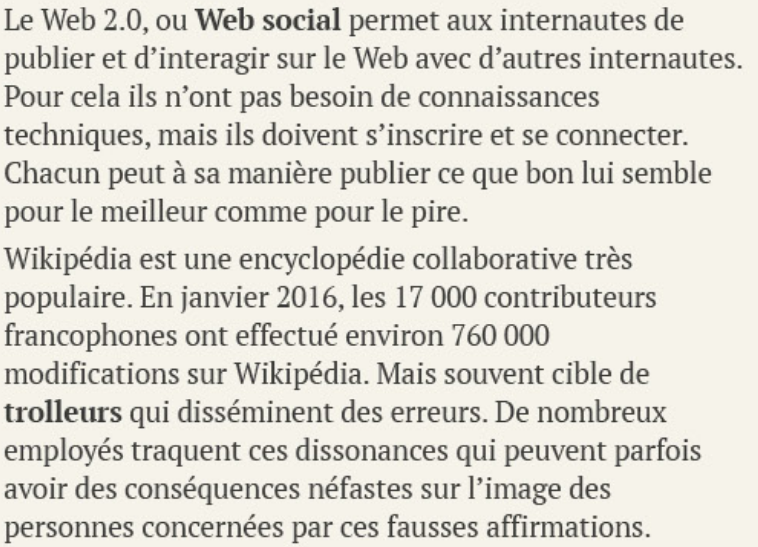
\includegraphics[width=9cm]{web_2.0.png}
  \end{center}\columnbreak

  \vspace*{-3mm}

  \begin{enumerate}
    \item Qu'est-ce qu'un troll/trolleur ?\rep{4}
    \item Citer un avantage de l'édition collaborative.\rep{4}
    \item En citer un inconvénient.\rep{4}
  \end{enumerate}
\end{multicols}

\bigskip

\textbf{Document 2 -- Législation encadrant les publications sur le Web} 

\smallskip

\begin{multicols}{2}
  \begin{enumerate}[resume]
    \item Que dit l'article 1 de la loi du 29 juillet 1881 sur la liberté de la presse ?\rep{5}
    \item À quel article de la Déclaration des droits de l'homme et du citoyen cet article fait-il écho ?\rep{5}
  \end{enumerate}

  \begin{center}
    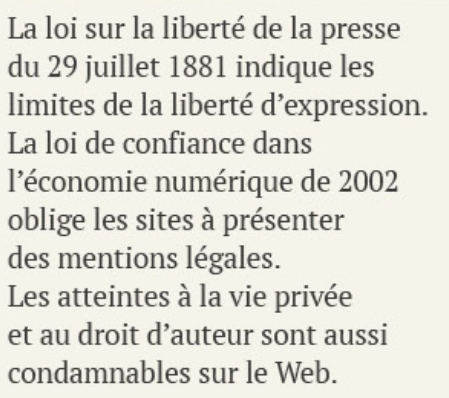
\includegraphics[width=7cm]{legislation_publications_web.png}
  \end{center}
\end{multicols}

\begin{enumerate}
  \setcounter{enumi}{5}
\item Que dit la loi pour la confiance dans l'économie numérique en matière de publicité électronique (par email par exemple) ?\rep{6}
\end{enumerate}

\pagebreak

\textbf{Document 3 -- Personnalisation de l'expérience utilisateur} 

\medskip

\begin{multicols}{2}
  \begin{center}
    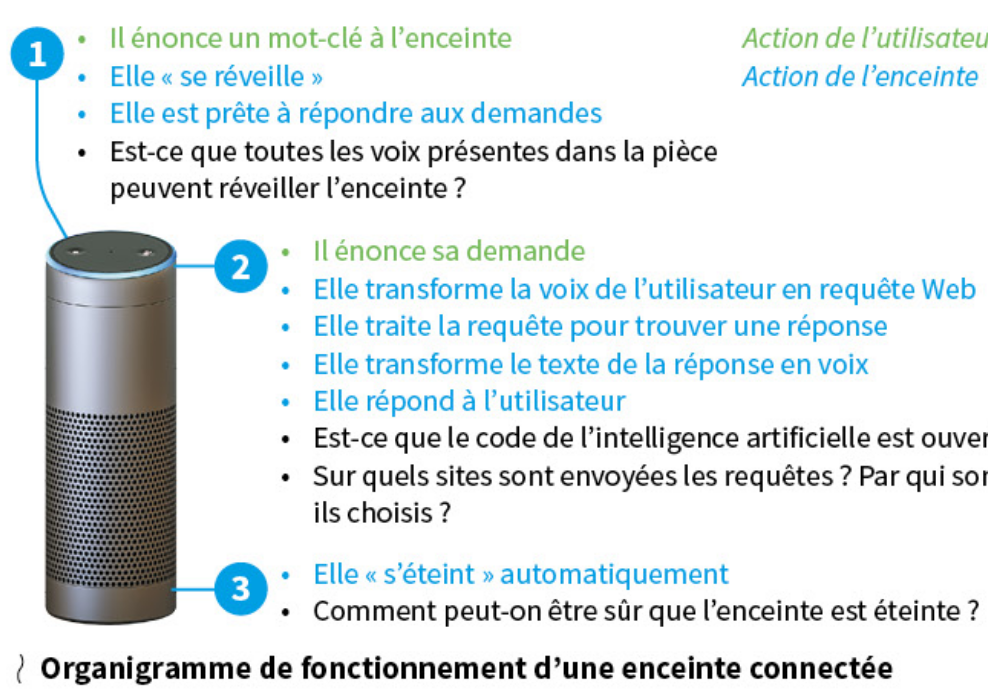
\includegraphics[width=9cm]{enceinte_connectee.png} 
  \end{center}\columnbreak
  \begin{enumerate}[resume]
    \item Donner deux exemples d'enceintes connectées.\rep{4}
    \item Donner un avantage de posséder une enceinte connectée.\rep{4}
    \item Donner un inconvénient d'en posséder une en citant un fait divers récent.\rep{4}
  \end{enumerate}
\end{multicols}

\bigskip

\textbf{Document 4 -- Retenir l'attention des internautes} 

\begin{center}
  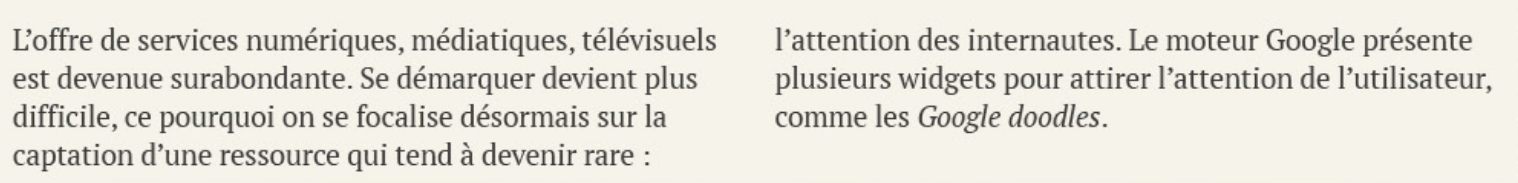
\includegraphics[width=16cm]{attention_internautes.png}
\end{center}

\begin{enumerate}[resume]
  \setcounter{enumi}{9}
  \item Qu'est-ce qu'un \textit{Google Doodle} ?\rep{3}
  \item Chercher la définition d'\textit{infinite scroll}.\rep{3}
  \item Q'est-ce qu'une \textit{notification push} ?\rep{3}
\end{enumerate}

\bigskip

\textbf{Document 5 -- En 2019, les 30 ans de l'invention du Web} 

\begin{center}
  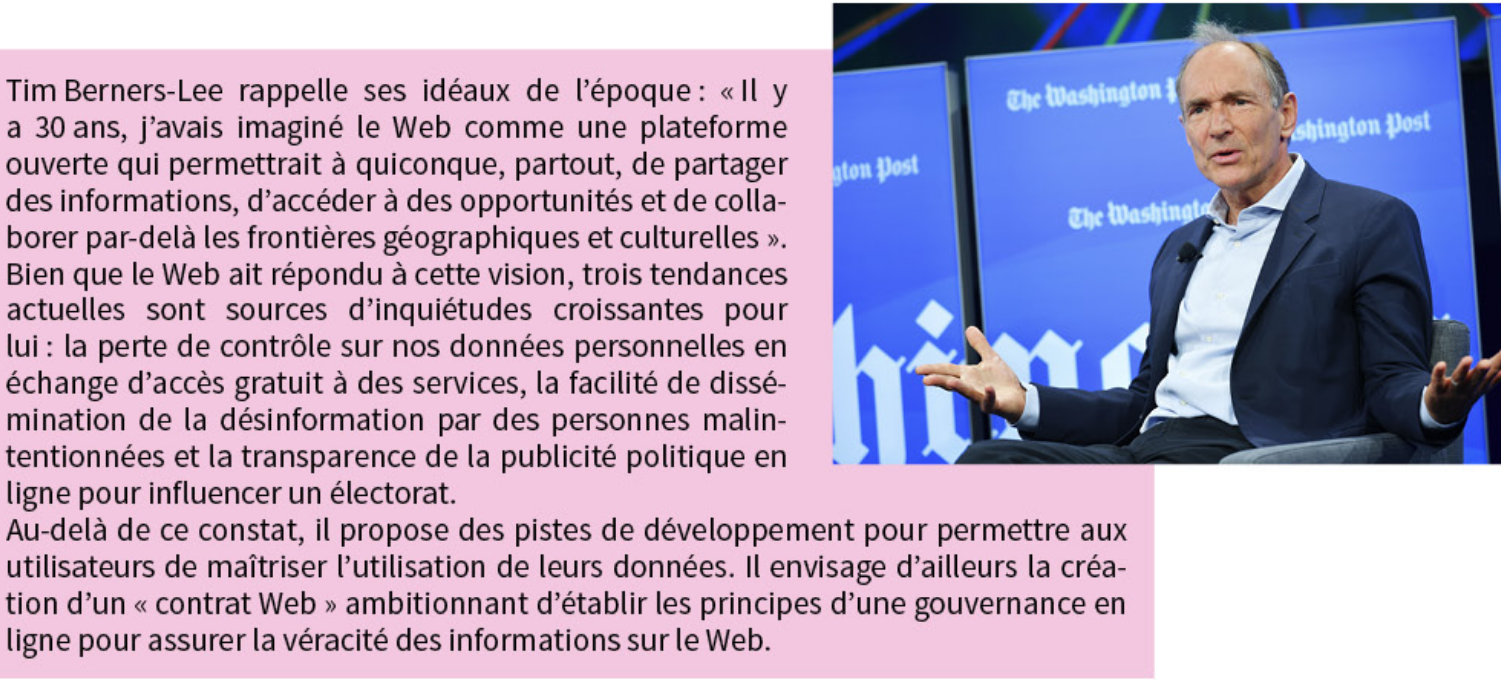
\includegraphics[width=16cm]{tim_berners-lee_entrevue_washington_post.png}
\end{center}

\begin{enumerate}
  \setcounter{enumi}{12}
  \item Le document ci-dessus est tiré d'une entrevue accordée par Tim Berners-Lee au Washington Post. Quelles inquiétudes Tim Berners-Lee partage-t-il ?\rep{6}
  \item On retrouve parfois ce message sur le mur de certains utilisateurs du réseau social Facebook :

    \begin{center}
      \textit{N'oubliez pas la date limite demain !!! Tout ce que vous avez publié devient public à partir de demain. Même les messages qui ont été supprimés ou les photos qui n'ont pas été autorisées. Ça ne coûte rien pour une simple copie et coller, mieux vaut que désolé. Channel 13 news a parlé du changement dans la politique de protection de la vie privée de Facebook. Je ne donne à Facebook ni à aucune entité associée à Facebook l'autorisation d'utiliser mes photos, informations, messages ou publications, à la fois passé et futur. Avec cette déclaration, je fais remarquer à Facebook qu'il est strictement interdit de divulguer, de copier, de distribuer ou de prendre toute autre action contre moi en fonction de ce profil et / ou de son contenu. Le contenu de ce profil est des informations privées et confidentielles. La violation de la vie privée peut être punie par la loi (UCC 1-308-1 1 308-103 et le statut de Rome).}
    \end{center}

    \begin{enumerate}[resume]
      \item Pourquoi ces utilisateurs publient-ils ce message ?\rep{4}
      \item Que penser de son utilité ?\rep{4}
    \end{enumerate}
  \item Résumer en quelques phrases le scandale Facebook-Cambridge Analytica.\rep{4}
\end{enumerate}
\end{document}
